\documentclass{article}

% Math
\usepackage{amsmath} % for matrices
\usepackage{amsfonts}
\usepackage{amssymb}

% Images
 \usepackage{graphicx}

% Code typesetting
\usepackage{listings}
\usepackage{color}
\definecolor{dkgreen}{rgb}{0,0.6,0}
\definecolor{gray}{rgb}{0.5,0.5,0.5}
\definecolor{mauve}{rgb}{0.58,0,0.82}

\lstset{frame=tb,
  language=Python,
  aboveskip=3mm,
  belowskip=3mm,
  showstringspaces=false,
  columns=flexible,
  basicstyle={\small\ttfamily},
  numbers=none,
  %numberstyle=\tiny\color{gray},
  %keywordstyle=\color{blue},
 % commentstyle=\color{dkgreen},
  %stringstyle=\color{mauve},
  breaklines=true,
  breakatwhitespace=true,
  tabsize=3
}

% Hyperlinks \href:
\usepackage[colorlinks=true, urlcolor=blue, linkcolor=red]{hyperref}

% Table:
\usepackage[table,xcdraw]{xcolor}
% Beamer presentation requires \usepackage{colortbl} instead of \usepackage[table,xcdraw]{xcolor}
\usepackage[normalem]{ulem}
\useunder{\uline}{\ul}{}

% Comments / todo's:
\newcommand{\todo}[1]{\textcolor{gray}{\textbf{Todo:} #1}}
\newcommand{\remark}[1]{\textcolor{red}{\textbf{\newline Remark:} \newline #1 \newline}}

% Dyanamic urls:
\newcommand{\oaaxweb}{\href{https://oaax.org}{https://oaax.org}}
\newcommand{\oaaxgit}{\href{https://github.com/oaax-standard}{https://github.com/oaax-standard}}

\begin{document}

\title{Towards an open and standardized mechanism for deploying ML/AI models to hardware accelerators.}
\author{The OAAX consortium.}
\date{May 2024}
\maketitle

\begin{abstract}
This position paper introduces the first outlines of OAAX; a novel initiative to make AI model deployment easier and more accessible. OAAX is composed of a set of standardized computing processes (conversion toolchains) and interfaces (APIs / ABIs) that are jointly aimed to make it extremely easy for developers to run trained AI models on novel AI accelerators  (NPUs, FPUs, GPUs, etc., generally referred to as XPUs). We present the high level technical structure of OAAX, consisting of OAAX conversion toolchain(s), which convert hardware agnostic model specifications (i.e., a model specification in a common format such as ONNX) to a hardware specific model specification, and OAAX runtimes; highly efficient modular blocks that are easily integrated within a larger ML/AI pipeline running on an edge device. From a developer perspective, OAAX enables moving between various accelerator targets with minimal effort such that any application developer can select the chipset best suited for their applications without incurring large software development cost. We outline the components of OAAX, provide examples, and discuss its limitations. In this position paper we also discuss the envisioned organization of the OAAX consortium and actively invite members of the community to contribute.
\end{abstract}

\tableofcontents

\section{Introduction}

The Open, AI Accelerator (OAAX) initiative,  (see, \oaaxweb) intends to provide an easy-to-use, easy-to-expand, \emph{standardized} methodology of adopting specific (edge) AI accelerators such as NPUs, GPUs, FPUs or the like---we will call them XPUs throughout this position paper---in edge AI / ML applications. As such, OAAX aims to alleviate the three most prominent hurdles towards using (Vision) edge AI solutions as identified in the March 2024 Edge AI + Vision alliance developer survey \cite{EVS}:
\begin{enumerate}
\item ``... the hardware required is too costly'' (60\%),
\item ``... the development (software) is too costly'' (57\%), and,
\item ``... the hardware required is too power hungry'' (48\%).
\end{enumerate}
By standardizing and effectively decoupling AI/ML pipeline software development from XPU acceleration, OAAX makes it easier to switch to more cost or power efficient AI specific hardware and reduces overal pipeline development time.

OAAX is designed to make it easy to take a \emph{trained} AI model and execute it (i.e., generate inferences from that model) on novel (edge) AI hardware. For AI solution developers (ISVs) OAAX should make it easy to reap the benefits of the new chipsets that are becoming available rapidly without having to worry about the target hardware when setting up and testing their initial AI pipeline. For those designing and bringing to the market new XPUs, OAAX is aimed at lowering the barriers of entry by providing a unified way in which -- if adhered to -- any developer can easily utilize the advantages of the newly introduced XPU.

Please note that the aims of this position paper are threefold:
\begin{enumerate}
\item First, we want to detail why we feel a standard mechanism for the deployment of ML/AI models, developed and maintained by our edge AI community, is useful.
\item Second, we want to provide a rough first outline of such a standard. Currently, this should merely be regarded as a \emph{proposal}; details of the standard should be developed by the community in several focus groups and joint working groups.
\item Third, we want to sketch the community driven approach we think is necessary to make the standard a success. Starting from the first focus group, to, potentially, reaching the status of an accredited international standard.
\end{enumerate}
Specifically on the last point, we are currently (May 2024) actively inviting those interested to join our first focus group(s) (please see Section \ref{sec:oaax-organization} below for details regarding the organizational structure). Please contact us at \oaaxweb ~when you are interested in contributing to the development of OAAX.

\subsection{The aims OAAX}

At a high level, OAAX aims to make it easier to develop edge AI applications that reap the benefits from newly introduced XPUs. More specifically,

For \emph{AI solution developers}, OAAX aims to:
\begin{itemize}
\item Provide a unified way of \emph{converting} a trained AI/Ml model that is available in a standardized, generic, format to a specific format that runs on the target hardware. Standardizing the conversion process saves valuable development time whilst it removes the burden of having to learn a new software ecosystem, toolchain, and -- in some cases -- model training tools required to reap the benefits of a specific XPU. It makes models truly portable.
\item Provide a unified way of \emph{executing} the specific model on the target hardware. I.e., OAAX provides a standardized ABI/API to load a model, pass input data to this model, run the inference, and retrieve the model output. This standardization makes that developer can build the surrounding pipeline / application without having to worry about the particularities of the chipset used for AI/ML inferences once the application is deployed. This makes pipelines XPU independent.
\end{itemize}

Jointly, the above allows AI solution developers to easily move between different hardware targets and reap the fruits of new developments in accelerator design that benefit their use case (i.e., use more cost efficient or energy efficient chipsets).

For \emph{manufacturers} of XPUs, OAAX aims to:
\begin{itemize}
\item Provide a unified way of allowing ``access'' to their hardware. By adopting OAAX, there is a single point of entry for developers looking to test and embrace the new hardware. This lowers barriers of entrance to the market.
\item Reduce the need to extensively develop one's own software ecosystem. By adopting OAAX, higher level software tools and ecosystems can easily incorporate new hardware without the need for the manufacturer of the accelerator to provide all the parts of a full AI/ML pipeline: accelerator manufacturers can simply focus on their hardware and the core software components needed to run an AI model on their hardware.\footnote{At this moment in time, some individual XPU makers, provide an extensive software ecosystem which effectively locks in application developers by needlessly inflating development costs associated with switching hardware. In our view, in the long run, this hinders overall market growth and leads to suboptimal applications. OAAX is, in part, designed to be a fully open -- both in terms of code and in terms of governance -- response to undesirable lock in.} This increases the overal market size.
\end{itemize}

Note that OAAX should be designed for maximum flexibility for the XPU manufacturer to convert a trained AI model to their preferred format and to -- if desirable -- keep toolchains, or other core bits of software that are deemed business valuable, proprietary by simply providing compiled versions or version that are accessible in the cloud.

\subsection{The scope of OAAX}

Currently, OAAX focusses on providing a unified method of \emph{accelerating} (i.e., (partly) moving to the XPU) trained AI/ML models. \emph{Models}, in our context, are simply (mathematical) functions that are specified using some hardware agnostic description standard: we adopt ONNX \cite{ONNX} for this purpose in our first implementation of OAAX.\footnote{In recent years ONNX has grown to include not just the implementation agnostic model specification, but also a set of model optimization tools and even model runtimes, we discuss relationships of OAAX to these extended initiatives in the related work section of this position paper. At this point in the text we treat ONNX simply as a standardized file format to encode a set of computations.}. At its core, ONNX is simply a standardized (file) format used to express which computations (or ``operations''), on which data, need to be carried out in which order. ONNX describes the computations start-to-end by specifying a Directed Acyclic Graph (DAG), in which nodes represent operations, and edges represent tensors ``flowing'' from one computation to the other. Throughout we assume that AI/ML models have one or multiple typed tensors as input ($I$), and  one or multiple typed tensors as output ($O$) .

OAAX does \emph{not} facilitate using the accelerator for application/vertical specific tasks such as decoding of a video stream or fast Fourier transform of a vibration sensor; such operations might be performed well by a specific XPU, but they do not fall into the scope of the initial  specification which is meant to be application agnostic. Also, OAAX does \emph{not} concern model training: we assume the trained model is available in ONNX format.\footnote{Our specification of OAAX toolchains does allow individual XPU makers to include training or validation data into the conversion process from generic to specific model specification as is often needed for (e.g.,) effective quantization.}

The diagram below provides a high level abstraction of a common edge ML/AI pipeline found in many applications in which sensor data is,
\begin{enumerate}
\item pre-processed,
\item fed to an AI/ML model for inference,
\item its results are post-processed, and,
\item the final output is visualized.
\end{enumerate}

Within OAAX we assume such a pipeline runs on a generic CPU (multiple architectures will be supported), whereas the AI model --- or, in some cases, individual operations within the AI model, depending on the accelerator manufacturer's choice --- is \emph{accelerated} on the XPU using the generic interface of OAAX runtime.\footnote{Note that we also provide CPU based runtimes to make sure that OAAX can also be used on non-XPU enabled hardware for development purposes.} Figure \ref{fig-pipeline} below provides a simple overview of the initial scope of OAAX within the larger AI/ML pipeline. OAAX allows for the block labelled ``AI/ML model'' to be easily moved from CPU to virtually any XPU by providing \emph{a)} the mechanism to convert a generic model description to a specific model description suited for execution on the XPU, and \emph{b)} providing a standardized interface to access the XPU from the process running on the CPU.

\begin{figure} [!htbp]
\centering
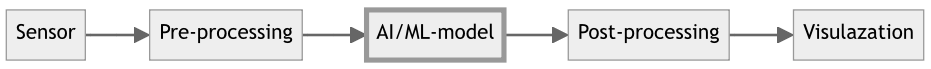
\includegraphics[width=0.9\textwidth]{img/pipeline}
\caption{Overview of a typical AI/ML pipeline from sensor to application. Although many production pipelines will have more moving parts --- potentially multiple models, aggregation, etc. --- at a high level it is very often possible to isolate one (or multiple) AI/ML models within the pipeline that would benefit from XPU acceleration.}
\label{fig-pipeline}
\end{figure}

\subsection{High level implementation}

At a very high level, the envisioned specification of OAAX is surprisingly simple. As a starting point, we assume a (trained) AI model $\mathcal{M}$ is available in ONNX format. Hence, there is access to a generic, deployment independent, description of the function that is implemented by AI/ML model: $\mathcal{M} \colon I \to O$.  From this starting point we postulate that  the following two steps are necessary and sufficient to accelerate an AI/ML model (or parts thereof\footnote{When thinking about models as a DAG, it is easy to see that a subgraph of the DAG is a DAG itself. As many XPU only support a small set of operations --- smaller than the most current ONNX standard operations set --- often only a subgraph of the original graph is meaningfully accelerated.}) within the larger pipeline:

\begin{enumerate}
\item \emph{Conversion} of the model's generic ONNX model specification to a format that can run on the accelerator. Note that the result might itself be in ONNX format (for example when operations are accelerated one-by-one by the runtime, see below), or the result might be a totally proprietary binary. The core insight is that there is a "conversion" step necessary from generic model description to a model description that is specific and can be (partly) accelerated using the XPU of interest. For the conversion step OAAX merely provides a unified way of going from ONNX to the target's specification (whatever this might be) including standardized error handling and formatting. We call the conversion process the \textbf{OAAX toolchain} and formally the process itself is simply a function that maps the generic model specification into an XPU specific one: $f \colon \mathcal{M} \to \mathcal{M}_{xpu}$.
\item \emph{Running} the specific model specification, i.e., generating inferences. Once a specific model specification is available---after conversion---we simply need a unified way to, from a process running on the CPU, pass data to the model, execute its computation, and return the results. We call this the \textbf{OAAX runtime.} Note that the OAAX runtime itself is a process running on the host CPU that is responsible for all interactions with the XPU. Abstractly, the runtime computes $O = \mathcal{M}_{xpu}(I)$.
\end{enumerate}

The above are deliberately---and contrary to some other attempts in this space---two separate steps: The first of the two steps can be executed anywhere: the conversion of a generic AI model to the target specific model can be done in the cloud, on your local machine, or (in the future) using some hosted conversion service. It is often done only once per (edge) AI target. The second step is executed, repeatedly, on the (fleet of) edge device(s) that runs the AI/ML pipeline (see \ref{fig-pipeline}). Thus, conversion and running are often two separate processes, carried out on physically separate devices.

Given the availability of a standardized method---OAAX---for sharing both steps with the larger developer community, it is easy for developers to adopt a new XPU into their edge AI applications. To adopt a new XPU, a developer simply:
\begin{enumerate}
\item Executes the \textbf{OAAX toolchain}, on whichever machine they prefer, to generate the XPU specific model $\mathcal{M}_{xpu}$. This step eliminates having to learn XPU specific conversion or training tools
\item ``Swaps'' the \textbf{OAAX runtime} in the larger application pipeline to match the selected hardware. Given a single interface for each and every runtime,\footnote{Including runtimes that run on CPUs, and hence allow for easy local evaluation if no XPUs are readily available.} this step eliminates any re-engineering necessary to adopt the new XPU.
\end{enumerate}

As a first implementation of OAAX we make a number of specific technical choices. For the \textbf{OAAX toolchain} we use pre-defined Docker images. Usage of Docker images to implement the  \textbf{OAAX toolchain} allows maximum flexibility for those contributing toolchains to use whatever conversion tools and dependencies they need inside the image. By simply standardizing the high level interactions with the container, we provide a unified method of model conversion while abstracting away any implementation details. On top of this, Docker images are easily managed and distributed and can be executed cross platform. For the  \textbf{OAAX runtime} we allow any (compiled) format, as long as there is a unified runtime ABI (shared library) available such that the runtime can be integrated in \texttt{C++} code. This should allow any low level application developer to utilize the OAAX runtime (and will allow for higher level (e.g., \texttt{Python} tools to be built on top of the lower-level runtime(s).

\subsection{Organization of this position paper}

The remainder of this position paper is organized as follows; first, we detail the usage of OAAX from a user / developer perspective. Next, we describe the core specification of OAAX (the latest version of which can always be found at \oaaxgit). Subsequently, we discuss the organization of the consortium and the ways in which the community can contribute to moving OAAX forward. Finally, we discuss relationships to other open and commercial projects that also aim, in one way or another, to make (edge) AI development and deployment easier. We close off with a discussion of the known limitations of OAAX.

\section{OAAX from a user / developer perspective}

Here we provide a few simple and self-contained\footnote{In the body text we focus on the core lines of code that illustrate the utility of OAAX, working code examples our found on the OAAX github pages, \oaaxgit.} examples of how to use the OAAX standard to switch from a CPU\footnote{We obviously provide a CPU only implementation of the OAAX Runtime as a CPU is a member of the set of XPUs.} only implementation of a (simplified) AI pipeline to one in which the model is accelerated using a Hailo Accelerator (using an initial implementation of OAAX to move over to this XPU). %For the sake of example, we use a simple pre-trained YoloV5 vision model in ONNX format (see \oaaxgit for details).

\subsection{Getting started from \texttt{C++}}

We start our example by assuming there is a hardware agnostic model file, \texttt{model-generic.onnx}, available to the user. We first show how to use the OAAX toolchain image to convert the hardware-agnostic model to a XPU specific model, \texttt{model-xpu.oaax}. Subsequently we show how to load the associated OAAX XPU runtime using \texttt{C++} and use it to generate inferences.

\subsubsection{Model Conversion}

In this section we show how to, from the command line, run the OAAX toolchain to transform the generic \texttt{model-generic.onnx} into a specific version of this model that can be run on the targeted accelerator. Given that the docker image has been downloaded to the local machine by the user, it suffices to run the following command:

\begin{lstlisting}
> ls
model-generic.onnx

> docker run -v $pwd:/root/model  oaax-xpu-toolchain:latest /root/model/model-generic.onnx /root/model/
> ls
model-generic.onnx
model-xpu.oaax
conversion-log.json
\end{lstlisting}

The workhorse of the above is clearly the \texttt{docker run} call which runs the (content of) the container once. We provide the following arguments:
\begin{itemize}
\item \texttt{-v \$pwd:/root/model} The \texttt{-v} flag for Docker run sets up a shared files system between the docker and the host in the pre-specified location and thus allows for the model file to be accessed from the container and for the output to be written to the local file system.
\item \texttt{/root/model/model.onnx} The path to the input file. Note that, depending on the XPU manufacturers specification, this can simply be a \texttt{.onnx} file, or it can be a \texttt{.zip} file containing the generic model description in ONNX and additional files for model conversion (i.e., validation examples used when quantizing the model).
\item \texttt{/root/model/model-xpu.oaax} The location and name of the output file. Users are free to choose the naming convention of the specific model file that is created.
\end{itemize}

The container should always produce the document \texttt{conversion-log.json}; this file should contain the conversion log containing human and machine readable conversion steps, and potential error messages. If conversion succeeds --- and thus the \texttt{errors} key of the \texttt{conversion-log.json} file is empty---the container will also produce a the xpu specific model file under the user provided name. We provide more details regarding the values in the \texttt{conversion-log.json} file and the possible input in our description of OAAX in Section \ref{sec:oaax-outline}. However, exact details of the format and data in the conversion-log file, for example whether it should contain structured information regarding the properties of the model, should be specified by the community as a whole.\footnote{In our current internal implementation of OAAX we also use mime-types to specify the output model format of the toolchain; using mime-types for this purposes is a technical detail that can be debated in the upcoming focus groups intended to further specify OAAX.}

\subsubsection{Loading the OAAX runtime}

When interacting with the OAAX runtime using \texttt{C/C++} on an edge device the application developer will need to load the XPU specific runtime into their project by including the correct shared library file:

\begin{lstlisting}
// Load the runtime library
handle = dlopen("./libRuntimeLibrary.so", RTLD_NOW);

// Load each runtime function one at a time
runtime_initialization_t runtime_initialization = (runtime_initialization_t)dlsym(handle, "runtime_initialization");
// ...
runtime_inference_execution_t runtime_inference_execution = (runtime_inference_execution_t) dlsym(handle, "runtime_inference_execution");
runtime_destruction_t runtime_destruction = (runtime_destruction_t) dlsym(handle, "runtime_destruction");
\end{lstlisting}

\subsubsection{Initializing the runtime}

Before starting to use XPU runtime for inference, the runtime needs to connect to the XPU, allocate resources, load the optimized model, etc.
That's achieved by calling the two functions below:

\begin{lstlisting}
// initialize runtime environment
if (runtime_initialization()) {
    print_error_message(runtime_error_message());
    dlclose(handle);
    return 1;
}

// load model
const char *file_path = model_path;
if (runtime_model_loading(file_path)) {
    print_error_message(runtime_error_message());
    dlclose(handle);
    return 1;
}
\end{lstlisting}

\subsubsection{Generating inferences}

Once the model file is available (the result from the toolchain), and the correct shared library file has been loaded, the core code necessary to run inferences while benefiting form the XPU is follows:

\begin{lstlisting}
// The input_tensors and output_tensors will contain the model input and output values.
tensors_struct input_tensors, output_tensors;
while(1){
    // Start inference on the input tensors
    if (runtime_inference_execution(&input_tensors, &output_tensors)) {
        print_error_message(runtime_error_message());
        break;
    }
    // here, you can use the model output tensors
    // ...

    // instruct the runtime to cleanup any intermediate results after we're done with the output tensors.
    if (runtime_inference_cleanup()) {
        print_error_message(runtime_error_message());
        break;
    }
}

// finalize runtime environment
if (runtime_destruction()) {
    print_error_message(runtime_error_message());
    dlclose(handle);
    return 1;
}
\end{lstlisting}

A complete and executable example of the above can be found int the OAAX github: \oaaxgit.

\newpage
\section{An outline of OAAX}
\label{sec:oaax-outline}

\remark{The current discussion of OAAX reflects our current, first, example implementation. We are currently actively looking to seek the community to refine the specification in a number of focus groups planned summer 2024.}

In this section we provide a first, rough, outline of OAAX, including details regarding the I/O of the toolchain and the signature of the Runtime (i.e., the functions it needs to expose for its users).

\subsection{OAAX Toolchains}

We start by detailing the input and output to the \textbf{OAAX Toolchain}. As demonstrated before, the toolchain is implemented as an easy to distribute Docker image; at the end of this section we provide an example of core parts of the Dockerfile needed to create the image. However, the overall design philosophy for the toolchain image is to impose as little restrictions as possible: it is up to the developer implementing the toolchain container to choose its external structure, its permitted input files, and the resulting output file format(s).

\subsubsection{Input to the Docker Container}

As discussed above, the only input to the Docker container is a file. This could be a model file in \texttt{onnx} format, but, alternatively for those XPU manufacturers who wish to use validation or training data to optimize model conversion for their chip, could be a \texttt{.zip} archive containing the model file and any additionally necessary files as specified by the XPU manufacturer in the documentation of the contributed XPU container.\footnote{Again, we stress that the discussion here is merely a first proposal; we might --- as a community -- decide to enforce more structure on the container specification.}.

\subsubsection{Output from the Docker Container}

The Docker container effectively writes out two files:
\begin{enumerate}
\item The model file. This can be either a \texttt{.onnx} file, a target specific binary, or anything the XPU manufacturer chooses to provide a device specific model description ($ \mathcal{M}_{xpu}$).
\item A conversion log file, called \texttt{conversion-log.json}. This file contains information regarding the conversion, potential model information, suggestions, errors, etc. The exact format needs specification, but we envision the \texttt{json} to contain:
	\begin{itemize}
		\item Meta data regarding the model.
		\item Human readable messages regarding the model conversion and toolchain documentation aimed at improving the conversion process.
		\item Computer readable error codes in case the conversion fails.
	\end{itemize}
\end{enumerate}

\subsubsection{Example of a Dockerfile}
As mentioned before, the conversion toolchain expects two parameters: the path of the input model, and the output directory where it can save the results artifacts. Therefore, it's sensible to define a script as an entrypoint of the Docker image that can trigger the rest of the conversion as illustrated in the Dockerfile below:
\begin{lstlisting}
ARG DEBIAN_FRONTEND=noninteractive
FROM ubuntu:22.04

WORKDIR /app

# You can for example install any dependencies the toolchain needs here
RUN #apt-get update -qq -y --fix-missing

COPY src/ /app/src/

ENTRYPOINT ["bash", "/app/src/run-toolchain.sh"]
\end{lstlisting}

\subsubsection{Contributing OAAX Toolchains}

We have collected a first implementation of an OAAX Toolchain for the Hailo accelerator in our github pages (see \oaaxgit). Copying this image should serve as a template for developers wishing to contribute their own XPU conversion toolchains.

\subsection{OAAX Runtimes}

In this section we provide more detail regarding the \textbf{OAAX runtime} which should be made available as a shared library file (see \oaaxgit for examples). We first provide a high level overview of the runtime. Next, we describe the content of the shared library file itself, before detailing the exposed functions.

\subsubsection{Overview of the runtime}

\begin{figure} [!htbp]
\centering
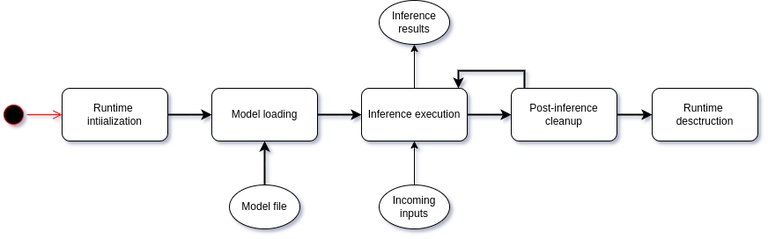
\includegraphics[width=0.9\textwidth]{img/runtime}
\caption{Overview of the interactions with the OAAX runtime: The runtime is initialized, after which the XPU specific model file(s) are loaded. Next, inferences can be generated by passing a list of tensors to the runtime. The runtime also facilitates cleanup and destruction.}
\label{fig-pipeline}
\end{figure}

The OAAX runtime effectively implements the following steps:\footnote{Where again we stress that this is merely intended to serve as a first suggestion.}

\begin{enumerate}
\item During the initialization step, the runtime is required to establish a connection with the XPU to ensure its usability, as well as initialize all components unrelated to the model.
\item The second stage involves loading the optimized model from a file. At this juncture, the runtime should be capable of executing inference on incoming inputs.
\item Inference run execution: Once the optimized model is loaded, the runtime will be fed incoming inputs one at a time and expected to return output results.
\item After completing each inference run, the runtime proceeds with post-run cleanup tasks. This may involve releasing any temporary resources allocated during the inference process, resetting internal states, or preparing for the next set of inference runs. Subsequently, the runtime either returns to step 3 to continue with further inference execution as necessary, or goes to the final stage.
\item Runtime resources destruction: It ensures that the runtime environment is properly cleaned up and ready for shutdown or further initialization if needed.
\end{enumerate}

\subsubsection{Shared Library file}

We make runtime available using shared library files. This allows a developer to include the XPU runtime in their edge AI project by simply ``swapping'' the included library; as the interface to the runtime is standardized -- i.e., the shared library file implements the same methods -- the surrounding code should not need any adaptation to move from one XPU\footnote{Readers should mentally include standard CPUs into the set of available XPUs; this allows OAAX to be used to develop a pipeline on a general purpose machine and subsequently, effortlessly, move it over to an edge device that includes a dedicated ML/AI accelerator.} to another.

\subsubsection{Runtime interface}

The runtime should provide an implementation of all functions listed below, which we split up in core functionality functions and utility functions:
\begin{itemize}
	\item Core functionality functions:
	\begin{itemize}
		\item \texttt{runtime\_initialization}: This stage involves the initialization of the runtime, ensuring all necessary components are properly set up and ready for operation.
		\item \texttt{runtime\_model\_loading}: During this stage, the runtime loads the model from storage or memory, preparing it for inference tasks.
		\item \texttt{runtime\_inference\_execution}: In this stage, the runtime executes the inference process, utilizing the loaded model to process input data and generate output predictions.
            \item \texttt{runtime\_destruction}: This stage marks the finalization of the runtime process, where any remaining resources are released, and the runtime environment is shut down gracefully.
	\end{itemize}
	\item Utility functions:
	\begin{itemize}
            \item \texttt{runtime\_inference\_cleanup}: After completing the inference tasks, the runtime performs cleanup operations, releasing any allocated resources and preparing for subsequent executions.
		\item \texttt{runtime\_name}: denotes the name of the runtime, serving as a useful identifier to distinguish it from other runtimes within the system.
		\item \texttt{runtime\_version}: This parameter signifies the version of the runtime, providing valuable information for tracking and ensuring compatibility with other components or systems.
		\item \texttt{runtime\_error\_message}: is utilized to retrieve the error message in case of a failure during any of the five stages of the runtime process. It serves as a valuable tool for diagnosing issues and troubleshooting problems encountered during runtime execution.
	\end{itemize}
\end{itemize}

\subsubsection{Contributing OAAX runtimes}

As for the OAAX toolchain, we provide a number of first implementations of the runtime in our github repository, see \oaaxgit.

\section{Additional tools and resources}

Next to the core implementation of the toolchain and runtime described above, we aim to build OAAX with a  number of tools and utilities to increase its value both for developers and for contributing XPU manufacturers. Here we list envisioned Python tools, skeleton implementations, utility toolchains, and testing tools separately.

\remark{At this point in time we simply list a number of desiderata; i.e., tools that we aim to develop within the OAAX ecosystem. However, specific working groups should contribute their own tools, and the first focus group discussions should be used to prioritize tool development.}

\subsection{Python tools}

Throughout this position paper we have demonstrated the core interactions with the runtime using the \texttt{C++} shared library (and hence we provide \texttt{C++} examples. We aim to develop a number of \texttt{Python} tools that allow for interactions with the OAAX XPU runtimes directly from \texttt{Python}. A first example of such a Python based interaction with the lower level \texttt{C++} OAAX runtime can already be found in our github: \oaaxgit. We aim to develop this further into a mature package allowing the \texttt{Python} developer community to easily integrate OAAX into their development process.

\subsection{Skeleton implementations}

We want to ensure that contributing OAAX toolchains and runtime, both by XPU manufacturers as well as by the community, is as easy as possible. As such we are looking to provide several skeleton implementations of the OAAX toolchain and runtime, each with utilities (one can imagine simple \texttt{Python} based utilities to check the submitted \texttt{.onnx} graph, inspect its operators, recognize specific model architectures, etc.).

\subsection{Utility toolchains}

Interestingly, OAAX ``ONNX-to-XPU'' toolchains can easily become part of a larger ecosystem of toolchains. For example, a simple container implementation of a toolchain which validates an ONNX graph and potentially changes its version would be well-sought after (and useful for model developers also outside of OAAX). Conversion toolchain containers from other model formats to ONNX, i.e., conversion from PyTorch of from TensorFlow to ONNX, would also provide a valuable contribution to OAAX (and to the edge AI community as a whole). Such model conversion from one-format-to-the-other is currently also supported by MMdnn \cite{MMdnn}.

\subsection{OAAX testing and profiling tools}

When OAAX matures, it will also prove a valuable ground for (automated) testing and profiling. XPU-contributed OAAX toolchains can easily be tested using a variety of common model architectures to validate the conversion process and ensure the newly contributed XPU supports the most sought after operators. OAAX could provide a breeding ground to ensure a standardized list of operators that minimally need to be supported for an XPU to be useful within the larger edge AI ecosystem.

Similarly, OAAX runtimes could easily be used to standardize model performance testing. Given a standardized set of trained models and input examples, a contributed OAAX runtime can be tested automatically by feeding the input to the runtime in a standardized way and monitoring the output accuracy, running speed, power consumption, etc. of the XPU. Thus, OAAX can provide the basic building block to develop an industry benchmark that XPU manufacturers can easily use to demonstrate the superiority of their hardware.

\section{The OAAX consortium organization}
\label{sec:oaax-organization}

In the sections above we have detailed the utilities of OAAX and we have tried to provide a high-level description of its first implementation. However, we are committed to make OAAX a community initiative which is not owned by a single XPU manufacturer or ISV but rather serves as an open community to jointly grow the field of edge AI by allowing the market to accelerate. To ensure community participation we describe our envisioned organizational structure, the (currently) envisioned end-goal, and we extend an invite for those interested to join our first focus groups.

\subsection{Envisioned organizational structure}

Although it will take time to mature the organization of OAAX, we envision building towards a structure that is akin to other successful standard in the Vision field such as ONVIF and ONNX. The ONVIF organization is mature and consist of the following bodies:

\begin{itemize}
\item \textbf{Steering Committee.} The Steering Committee is responsible for strategy and budgeting.
\item \textbf{Technical Committee.} The Technical Committee (TC) drives the development of the core specifications as well as the technical direction and roadmap.
\item \textbf{Technical Services Committee.} The Technical Services Committee (TSC) is responsible for the development of tools, testing and other auxiliary infrastructure.
\item \textbf{Communication Committee.} The Communication Committee is responsible for the organization’s external and internal communication.
\end{itemize}

The Technical Committee, the Technical Services Committee, and the Communication Committee will have several working groups (WGs) focussing on particular components of their tasks. We intend to move towards a similar organization structure to ensure continuity of OAAX.

\subsubsection{Envisioned process}

In parallel to building a mature organizational structure, we aim to start the process of creating an actual standard for (parts of) OAAX. At this moment in time we are in contact with ITU (\href{https://www.itu.int/en/ITU-T/studygroups/2017-2020/16/Pages/q5.aspx}{https://www.itu.int/en/ITU-T/studygroups/2017-2020/16/Pages/q5.aspx}) to aid us in this process and to coordinate the first focus groups to detail the first technical and organizational structures OAAX.

\subsection{Joining the first OAAX  focus groups}

While the above sketches a direction of the organization of OAAX, you can get involved straight away. We invite you to express your interest in joining our first focus group(s) -- or in the future joining any of the respective working groups -- by leaving your email at \oaaxweb.

\section{Limitations}

The first high level OAAX  description as provided in Section \ref{sec:oaax-outline} contains a number of known gaps or discussion points. We highlight a few points that will need attention when further developing the standard:

\begin{itemize}
\item \textbf{Model class / architecture support.} As model architectures --- and underlying operators --- are evolving rapidly, it is an open question whether or not OAAX should include specific (minimum) requirements regarding model architecture or operator support.
\item \textbf{(Exact) runtime timing.} As numerous edge AI deployments --- especially in an industrial setting --- will need mechanisms to exactly time model execution (and potentially abort if timing requirements are exceeded), it is likely that explicit timing of the OAAX runtime in a realtime OS will need more specification.
\item \textbf{Runtime memory management.} Although our first implementation provides a rudimentary mechanism to free up memory, efficient memory use between CPU and XPU, and sometimes even within the XPU (which might be dependent on the model choice) can be key to squeezing out the last bits of performance. OAAX should provide XPU manufacturers with all the tools the need to ensure their hardware is used to its fullest efficiency.
\item \textbf{Runtime behavior for multiple models.} In many applications an application developer will use multiple models, either in sequence or in parallel. Additionally some XPUs support sequential use of the hardware with multiple inputs, or otherwise batched inputs to the XPU. These technical details will need to be developed either inside of the OAAX runtime specification, or best-practices for the (e.g.,) parallel use of multiple OAAX runtimes will need to be documented.
\item \textbf{Runtime concurrency / asynchronous processing.} A number of XPUs thrive by having concurrent processing; currently OAAX runtimes are setup to generate (batches of) inferences one-by-one; we intend to more fully work out alternative, asynchronous, models of execution.
\item \textbf{XPU selection on target device.} We currently see multiple device manufacturers equipping edge AI devices with multiple different XPUs. Hence, it becomes key to control potentially multiple runtimes on a single device. Best practices dealing with such devices will need to be developed.
\end{itemize}

We are likely at this point overlooking a number of issues pertinent to both application developers (ISVs) and XPU manufacturers; we hope the first focus groups will allow us to more clearly define the limitations of the suggested approach and work on solutions in respective working groups.

\section{Related projects}

Given the large challenges that developers are facing to utilize new XPU efficiently, it is not surprise that there are many project which relate --- in one way or another --- to the development of OAAX. Table \ref{tab:overview} provides an overview. We aim to distill best-practices from each, and cordially invite contributors to any of these initiatives to collaborate on making edge AI more accessible.

\begin{table}[h!tp]
\begin{tabular}{lll}
\textbf{Name}          	 	& \textbf{Origin} & \textbf{Type}                         \\
OneAPI\cite{OneAPI}                  		& Intel           & Acceleration Library                  \\
CUDA X\cite{CUDAX}                 		 & NVIDIA          & Acceleration Library                  \\
ArmCompute Library\cite{ArmCompute}      	& Arm             & Acceleration Library                  \\
CoreML\cite{CoreML}                		 & Apple           & Acceleration Library                  \\
MMDNN\cite{MMdnn}         & Microsoft       & Conversion toolchain utility          \\
Paddle Paddle\cite{PaddlePaddle}           	& Paddle          & Model to binary                       \\
NCNN\cite{NCNN}                    		& Tencent         & Model to binary                       \\
MNN\cite{MNN}                     		& Alibaba         & Model to binary                       \\
ONNX Runtime\cite{ONNXRuntime}            	& Community       & Runtime                               \\
Triton Inference server\cite{Triton} 	& NVIDIA          & Runtime                               \\
Apache TVM\cite{TVM}              	& Community       & Runtime                               \\
Huggingface deploy\cite{Huggingface}      	& Hugging face    & Training platform specific deployment \\
Open VINO\cite{OpenVINO}              		& OpenVino        & Vendor specific toolchain + runtime   \\
Vision AI DevKit\cite{VisionAIDevKit}       		& Qualcomm        & Vendor specific toolchain + runtime   \\
Hailo  AI Suite\cite{Hailo}                 		& Hailo           & Vendor specific toolchain + runtime   \\
iMX OnnxRuntime\cite{iMX}       	& NXP             & Vendor specific toolchain + runtime
\end{tabular}
\caption{Overview of a selection of projects relating to OAAX. We see projects focussing on low level acceleration, model conversion, and model execution. Next to these projects we also see a number of vendor specific AI conversion and deployment projects.}
\label{tab:overview}
\end{table}

\section{Conclusions}

In this position paper we have tried to detail the need for an open standard to make it easier to develop edge AI applications that benefit from newly developed, edge AI specific, hardware (XPUs). Next, we sketched a first outline of such a standard (working examples of which can be found at \oaaxgit). Finally we discussed the envisioned future organization of the standard and discussed a number of known limitations and relationships to other projects.

At this moment in time (May 2024), we encourage readers who want to join in specifying OAAX and contributing to its community to join our first focus group(s) which will be planned in summer 2024. If you are interested, please do leave your email address at \oaaxweb.

\begin{thebibliography}{9}

\bibitem{EVS}
	 \href{https://www.edge-ai-vision.com/2023-computer-vision-and-perceptual-ai-developer-survey/}{https://www.edge-ai-vision.com/2023-computer-vision-and-perceptual-ai-developer-survey/}.
\bibitem{ONNX}
	 \href{https://onnx.ai/}{https://onnx.ai/}
\bibitem{MMdnn}
	\href{https://github.com/microsoft/MMdnn}{https://github.com/microsoft/MMdnn}
\bibitem{OneAPI}
	\href{https://www.intel.com/content/www/us/en/developer/tools/oneapi/overview.html}{https://www.intel.com/content/www/us/en/developer/tools/oneapi/overview.htm}
\bibitem{CUDAX}
	\href{https://www.nvidia.com/en-us/technologies/cuda-x/}{https://www.nvidia.com/en-us/technologies/cuda-x/}
\bibitem{ArmCompute}
	\href{https://www.arm.com/technologies/compute-library}{https://www.arm.com/technologies/compute-library}
\bibitem{CoreML}
	\href{https://developer.apple.com/documentation/coreml}{https://developer.apple.com/documentation/coreml}
\bibitem{PaddlePaddle}
	\href{https://github.com/PaddlePaddle/FastDeploy}{https://github.com/PaddlePaddle/FastDeploy}
\bibitem{NCNN}
	\href{https://github.com/Tencent/ncnn}{https://github.com/Tencent/ncnn}
\bibitem{MNN}
	\href{https://github.com/alibaba/MNN}{https://github.com/alibaba/MNN}
\bibitem{ONNXRuntime}
	\href{https://onnxruntime.ai/}{https://onnxruntime.ai/}
\bibitem{Triton}
	\href{https://developer.nvidia.com/triton-inference-server}{https://developer.nvidia.com/triton-inference-server}
\bibitem{TVM}
	\href{https://tvm.apache.org/}{https://tvm.apache.org/}
\bibitem{Huggingface}
	\href{https://github.com/orgs/huggingface/repositories?q=optimum}{https://github.com/orgs/huggingface/repositories?q=optimum}
\bibitem{OpenVINO}
	\href{https://github.com/openvinotoolkit/openvino}{https://github.com/openvinotoolkit/openvino}
\bibitem{VisionAIDevKit}
	\href{https://azure.github.io/Vision-AI-DevKit-Pages/}{https://azure.github.io/Vision-AI-DevKit-Pages/}
\bibitem{Hailo}
	\href{https://hailo.ai/products/hailo-software/hailo-ai-software-suite/}{https://hailo.ai/products/hailo-software/hailo-ai-software-suite/}
\bibitem{iMX}
	\href{https://github.com/nxp-imx/onnxruntime-imx}{https://github.com/nxp-imx/onnxruntime-imx}


\end{thebibliography}

\end{document}